\documentclass[../main/main.tex]{subfiles}

\newdate{date}{16}{10}{2019}

\begin{document}

\marginpar{ \textbf{Lecture 3.} \\  \displaydate{date}. \\ Compiled:  \today.}


\begin{figure}[h!]
\begin{minipage}[c]{0.5\linewidth}
\centering
\subfloat[][Coexistence plot.]{

\tikzset{every picture/.style={line width=0.75pt}} %set default line width to 0.75pt

\begin{tikzpicture}[x=0.75pt,y=0.75pt,yscale=-0.37,xscale=0.37]
%uncomment if require: \path (0,476); %set diagram left start at 0, and has height of 476

%Shape: Axis 2D [id:dp5951100625553807]
\draw  (12.61,425) -- (658.18,425)(77.17,2) -- (77.17,472) (651.18,420) -- (658.18,425) -- (651.18,430) (72.17,9) -- (77.17,2) -- (82.17,9)  ;
%Curve Lines [id:da6195327642832696]
\draw    (113.36,368.24) .. controls (230.74,358.36) and (344.5,208.49) .. (396.87,108.02) ;


%Curve Lines [id:da2126694468363458]
\draw    (292.51,257.9) .. controls (366.17,271.07) and (460.07,213.43) .. (532.3,164.02) ;


%Straight Lines [id:da7069592692010301]
\draw  [dash pattern={on 4.5pt off 4.5pt}]  (77.25,226.6) -- (320.4,228.21) ;


%Straight Lines [id:da5293875835625754]
\draw  [dash pattern={on 4.5pt off 4.5pt}]  (320.4,228.21) -- (318.6,424.19) ;


%Shape: Ellipse [id:dp08220348613655248]
\draw  [fill={rgb, 255:red, 0; green, 0; blue, 0 }  ,fill opacity=1 ] (313.19,228.21) .. controls (313.19,226.39) and (314.81,224.92) .. (316.8,224.92) .. controls (318.79,224.92) and (320.4,226.39) .. (320.4,228.21) .. controls (320.4,230.02) and (318.79,231.49) .. (316.8,231.49) .. controls (314.81,231.49) and (313.19,230.02) .. (313.19,228.21) -- cycle ;
%Shape: Ellipse [id:dp6417973207439449]
\draw  [fill={rgb, 255:red, 0; green, 0; blue, 0 }  ,fill opacity=1 ] (288.92,258.18) .. controls (288.74,256.37) and (290.21,254.78) .. (292.2,254.62) .. controls (294.18,254.46) and (295.93,255.8) .. (296.1,257.61) .. controls (296.27,259.42) and (294.8,261.02) .. (292.82,261.17) .. controls (290.83,261.33) and (289.09,259.99) .. (288.92,258.18) -- cycle ;

% Text Node
\draw (41.5,27.32) node [scale=1.5]  {$P$};
% Text Node
\draw (644.64,453.88) node [scale=1.5]  {$T$};
% Text Node
\draw (39.7,211.78) node [scale=1.5]  {$P_{o}$};
% Text Node
\draw (348.49,453.88) node [scale=1.5]  {$T_{n}$};


\end{tikzpicture}
    \label{fig:} }
\end{minipage}
\begin{minipage}[]{0.5\linewidth}
\centering
\subfloat[][Zoom of the coexistence line.]{

\tikzset{every picture/.style={line width=0.75pt}} %set default line width to 0.75pt

\begin{tikzpicture}[x=0.75pt,y=0.75pt,yscale=-0.37,xscale=0.37]
%uncomment if require: \path (0,459); %set diagram left start at 0, and has height of 459

%Shape: Axis 2D [id:dp5951100625553807]
\draw  (-0.5,413.21) -- (655.73,413.21)(65.12,2.77) -- (65.12,458.81) (648.73,408.21) -- (655.73,413.21) -- (648.73,418.21) (60.12,9.77) -- (65.12,2.77) -- (70.12,9.77)  ;
%Curve Lines [id:da6195327642832696]
\draw    (101.92,356.57) .. controls (221.23,346.83) and (336.87,199.14) .. (390.11,100.15) ;


%Straight Lines [id:da7069592692010301]
\draw  [dash pattern={on 4.5pt off 4.5pt}]  (65.2,217) -- (312.37,218.58) ;


%Straight Lines [id:da5293875835625754]
\draw  [dash pattern={on 4.5pt off 4.5pt}]  (312.37,218.58) -- (310.54,411.71) ;


%Shape: Ellipse [id:dp08220348613655248]
\draw  [fill={rgb, 255:red, 0; green, 0; blue, 0 }  ,fill opacity=1 ] (305.04,218.58) .. controls (305.04,216.79) and (306.68,215.34) .. (308.71,215.34) .. controls (310.73,215.34) and (312.37,216.79) .. (312.37,218.58) .. controls (312.37,220.37) and (310.73,221.82) .. (308.71,221.82) .. controls (306.68,221.82) and (305.04,220.37) .. (305.04,218.58) -- cycle ;
%Shape: Ellipse [id:dp6417973207439449]
\draw  [fill={rgb, 255:red, 0; green, 0; blue, 0 }  ,fill opacity=1 ] (344.61,168.59) .. controls (344.44,166.8) and (345.93,165.23) .. (347.95,165.08) .. controls (349.97,164.93) and (351.74,166.25) .. (351.92,168.03) .. controls (352.09,169.81) and (350.6,171.38) .. (348.58,171.54) .. controls (346.56,171.69) and (344.79,170.37) .. (344.61,168.59) -- cycle ;

% Text Node
\draw (28.87,20.62) node [scale=1.5]  {$P$};
% Text Node
\draw (641.96,439.96) node [scale=1.5]  {$T$};
% Text Node
\draw (27.03,202.39) node [scale=1.5]  {$P_{o}$};
% Text Node
\draw (340.92,440.96) node [scale=1.5]  {$T_{n}$};
% Text Node
\draw (302.38,197.52) node   {$a$};
% Text Node
\draw (333.58,148.83) node   {$b$};
% Text Node
\draw (184.9,130.98) node   {$1$};
% Text Node
\draw (425.36,255.95) node   {$2$};


\end{tikzpicture}
    \label{fig:3_1} }
\end{minipage}
\caption{\label{fig:} }
\end{figure}


\noindent We know that because they are on the cohexistence line
\begin{equation}
  \begin{cases}
   g_1^{(a)} = g_2^{(a)}\\
   g_1^{(b)} = g_2^{(b)}
  \end{cases}
\label{eq:}
\end{equation}
and, if they are close enough:
\begin{equation}
  \begin{cases}
  \dd[]{g_1} = g_1^{(b)} - g_1^{(a)} \\
  \dd[]{g_2} = g_2^{(b)} - g_2^{(a)}
  \end{cases}
\label{eq:}
\end{equation}
Therefore, the \emph{starting point} for \emph{Clausius-Clapeyron} is
\begin{equation}
  \Rightarrow \dd[]{g_1} =\dd[]{g_2}
  \label{eq:}
\end{equation}
Consider also
\begin{equation}
  \begin{cases}
   \dd[]{g_1} = -s_1 \dd[]{T} + v_1 \dd[]{P}   \\
   \dd[]{g_2} = -s_2 \dd[]{T} + v_2 \dd[]{P}
  \end{cases}
\label{eq:}
\end{equation}
taking the difference, one obtains
\begin{equation}
  -(s_2 - s_1) \dd[]{T} + (v_2 - v_1) \dd[]{P} = 0
  \label{eq:}
\end{equation}
The splope is called \textcolor{blue}{\textbf{Clausius-Clapeyron equation}}:
\begin{empheq}[box=\myyellowbox]{equation}
  \qty(\dv{P}{T} )_{coex} = \frac{(s_2-s_1)}{(v_2-v_1)} = \frac{\Delta s}{\Delta v}
  \label{eq:}
\end{empheq}

 Now, we go from gas to liquid (respectively region 1 and 2 in Figure \ref{fig:3_1}), we have:
\begin{equation}
  \qty(\dv{P}{T} )_{coex} = \frac{s_2 - s_1}{v_2 - v_1} \qquad \substack{ s_2 > s_1 \\ v_2 > v_1} \Rightarrow \qty(\dv{P}{T} )_{coex} > 0
  \label{eq:}
\end{equation}
Melt:
\begin{equation}
  \qty(\dv{P}{T} )_{coex} = \frac{\delta Q_{melt}}{T_{melt}\Delta v_{melt}} \qquad \delta Q_{melt} = Q_{liq} - Q_{solid} > 0
  \label{eq:}
\end{equation}
In general, \( v_{liq} > v_{solid} \) which implies \( \qty( \dd[]{P}/\dd[]{T}   )_{coex} > 0  \), but there are cases when \( v_{liq} < v_{solid} \) and \( \rho_{liq} > \rho _{solid} \) (for instance the \( H_2 0 \), or also Silicon and Germanium).

\section{Order parameter}
The \emph{order parameters} are macroscopic observable that are equal to zero above the critical temperature, and different from zero below:
\begin{equation}
O_p
  \begin{cases}
  \neq 0 & T<T_c \\
  = 0 & T \rightarrow T_c^-
  \end{cases}
\label{eq:}
\end{equation}
It reflects the symmetry of the system. Recall that, at \( T_c \) the system has a symmetry broken. Consider \emph{ferromagnetic system}, we have \( \va{M} \rightarrow \va{H}   \), while for \emph{ferro electric} we have \( \va{P} \rightarrow \va{E}   \). For \emph{liquid crystals} \( Q_{\alpha \beta } \rightarrow \va{E},\va{H}   \).

Consider the densities of liquid and gas, their difference is \( \Delta \rho = \rho _{l} - \rho _{g} \), that is \( \neq 0 \) for \( T \neq T_c \) but \( \rightarrow 0 \) when \( T \rightarrow T_c \) (see Figure \ref{fig:3_2}).


\begin{figure}[h!]
\begin{minipage}[c]{0.5\linewidth}
\centering
\subfloat[][]{
\tikzset{every picture/.style={line width=0.75pt}} %set default line width to 0.75pt

\begin{tikzpicture}[x=0.75pt,y=0.75pt,yscale=-0.37,xscale=0.37]
%uncomment if require: \path (0,476); %set diagram left start at 0, and has height of 476

%Shape: Axis 2D [id:dp5951100625553807]
\draw  (12.61,425) -- (658.18,425)(77.17,2) -- (77.17,472) (651.18,420) -- (658.18,425) -- (651.18,430) (72.17,9) -- (77.17,2) -- (82.17,9)  ;
%Curve Lines [id:da6195327642832696]
\draw    (240.5,190) .. controls (271.5,139) and (201.5,72) .. (140.5,147) ;


%Curve Lines [id:da2126694468363458]
\draw    (218.5,392) .. controls (452.5,368) and (404.5,179) .. (240.5,190) ;


%Straight Lines [id:da7069592692010301]
\draw  [dash pattern={on 4.5pt off 4.5pt}]  (77.25,208.6) -- (332.5,209) ;


%Straight Lines [id:da5293875835625754]
\draw  [dash pattern={on 4.5pt off 4.5pt}]  (332.5,209) -- (331.5,425) ;


%Shape: Ellipse [id:dp08220348613655248]
\draw  [fill={rgb, 255:red, 0; green, 0; blue, 0 }  ,fill opacity=1 ] (328.89,209) .. controls (328.89,207.18) and (330.51,205.71) .. (332.5,205.71) .. controls (334.49,205.71) and (336.11,207.18) .. (336.11,209) .. controls (336.11,210.82) and (334.49,212.29) .. (332.5,212.29) .. controls (330.51,212.29) and (328.89,210.82) .. (328.89,209) -- cycle ;

% Text Node
\draw (47.5,27.32) node [scale=1]  {$\rho $};
% Text Node
\draw (644.64,453.88) node [scale=1]  {$T$};
% Text Node
\draw (47,211.78) node [scale=1]  {$\rho _{c}$};
% Text Node
\draw (348.49,453.88) node [scale=1]  {$T_{c}$};
% Text Node
\draw (48,139.78) node [scale=1]  {$\rho _{l}$};
% Text Node
\draw (47,299.78) node [scale=1]  {$\rho _{g}$};


\end{tikzpicture}
    \label{fig:} }
\end{minipage}
\begin{minipage}[]{0.5\linewidth}
\centering
\subfloat[][]{
\tikzset{every picture/.style={line width=0.75pt}} %set default line width to 0.75pt

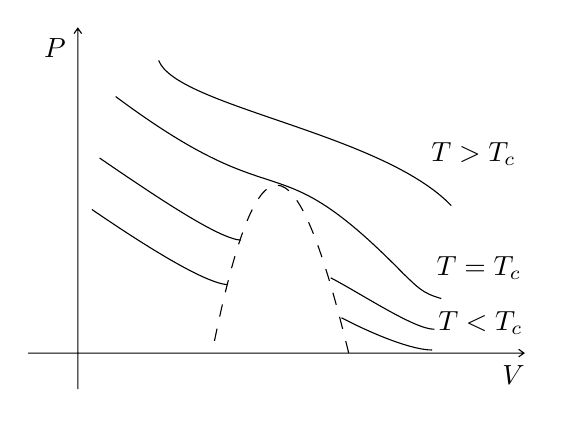
\begin{tikzpicture}[x=0.75pt,y=0.75pt,yscale=-0.37,xscale=0.37]
%uncomment if require: \path (0,476); %set diagram left start at 0, and has height of 476

%Shape: Axis 2D [id:dp5951100625553807]
\draw  (12.61,425) -- (658.18,425)(77.17,2) -- (77.17,472) (651.18,420) -- (658.18,425) -- (651.18,430) (72.17,9) -- (77.17,2) -- (82.17,9)  ;
%Curve Lines [id:da2126694468363458]
\draw    (563.5,233) .. controls (472.5,138) and (205.5,104) .. (182.5,44) ;


%Curve Lines [id:da8602998139648838]
\draw  [dash pattern={on 4.5pt off 4.5pt}]  (429.9,424.97) .. controls (359.9,136.97) and (310.9,129.97) .. (251.9,424.97) ;


%Shape: Boxed Bezier Curve [id:dp6932412254916785]
\draw    (501.5,322) .. controls (326.5,143) and (349.5,257) .. (126.5,91) ;


%Curve Lines [id:da8502267220518913]
\draw    (289.5,278) .. controls (260.5,276) and (181.5,223) .. (105.5,171) ;


%Curve Lines [id:da8746517244181468]
\draw    (272.5,336) .. controls (243.5,334) and (171.5,290) .. (95.5,238) ;


%Curve Lines [id:da4382617853232931]
\draw    (538.5,421) .. controls (512.5,421) and (462.5,401) .. (420.5,379) ;


%Curve Lines [id:da368608553657754]
\draw    (541.5,394) .. controls (515.5,394) and (448.5,349) .. (406.5,327) ;


%Curve Lines [id:da19861479220559797]
\draw    (550.5,354) .. controls (525.5,347) and (519.5,339) .. (501.5,322) ;



% Text Node
\draw (47.5,27.32) node [scale=1]  {$P$};
% Text Node
\draw (644.64,453.88) node [scale=1]  {$V$};
% Text Node
\draw (601.49,385.88) node [scale=1]  {$T< T_{c}$};
% Text Node
\draw (599.49,313.88) node [scale=1]  {$T=T_{c}$};
% Text Node
\draw (592.49,165.88) node [scale=1]  {$T >T_{c}$};


\end{tikzpicture}
    \label{fig:} }
\end{minipage}
\caption{\label{fig:3_2} Description}
\end{figure}
In Figure \ref{fig:3_3} is shown the behaviour for a ferromagnetic system.
\begin{figure}[h!]
\centering


\tikzset{every picture/.style={line width=0.75pt}} %set default line width to 0.75pt

\begin{tikzpicture}[x=0.75pt,y=0.75pt,yscale=-0.7,xscale=0.7]
%uncomment if require: \path (0,476); %set diagram left start at 0, and has height of 476

%Shape: Axis 2D [id:dp5951100625553807]
\draw  (6.61,238.94) -- (652.18,238.94)(72.5,3) -- (72.5,473) (645.18,233.94) -- (652.18,238.94) -- (645.18,243.94) (67.5,10) -- (72.5,3) -- (77.5,10)  ;
%Curve Lines [id:da2126694468363458]
\draw    (582.5,278.94) .. controls (367.5,268.94) and (237.5,380.94) .. (127.5,471.94) ;


%Curve Lines [id:da8099781123736827]
\draw    (583.5,216.94) .. controls (448.5,202.94) and (228.5,87.94) .. (151.5,33.94) ;


%Curve Lines [id:da6865648324380681]
\draw [color={rgb, 255:red, 255; green, 0; blue, 0 }  ,draw opacity=1 ]   (71.5,99.94) .. controls (315.5,126.94) and (361.5,332.94) .. (72.5,397.94) ;


%Shape: Circle [id:dp406793341592669]
\draw  [color={rgb, 255:red, 255; green, 0; blue, 0 }  ,draw opacity=1 ][fill={rgb, 255:red, 255; green, 0; blue, 0 }  ,fill opacity=1 ] (267.06,237.97) .. controls (267.06,235.23) and (269.28,233) .. (272.03,233) .. controls (274.77,233) and (277,235.23) .. (277,237.97) .. controls (277,240.72) and (274.77,242.94) .. (272.03,242.94) .. controls (269.28,242.94) and (267.06,240.72) .. (267.06,237.97) -- cycle ;

% Text Node
\draw (47.5,27.32) node [scale=1.5]  {$M$};
% Text Node
\draw (626.64,258.88) node [scale=1.5]  {$T$};
% Text Node
\draw (492.49,372.88) node [scale=1]  {$H< 0$};
% Text Node
\draw (559.49,254.88) node [scale=1]  {$H=0$};
% Text Node
\draw (489.49,94.88) node [scale=1]  {$H >0$};
% Text Node
\draw (292.49,215.88) node [scale=1,color={rgb, 255:red, 253; green, 0; blue, 0 }  ,opacity=1 ]  {$T_{c}$};

\end{tikzpicture}


\caption{\label{fig:3_3} Description.}
\end{figure}



\begin{figure}[h!]
\begin{minipage}[c]{0.5\linewidth}
\centering
\subfloat[][]{
\tikzset{every picture/.style={line width=0.75pt}} %set default line width to 0.75pt

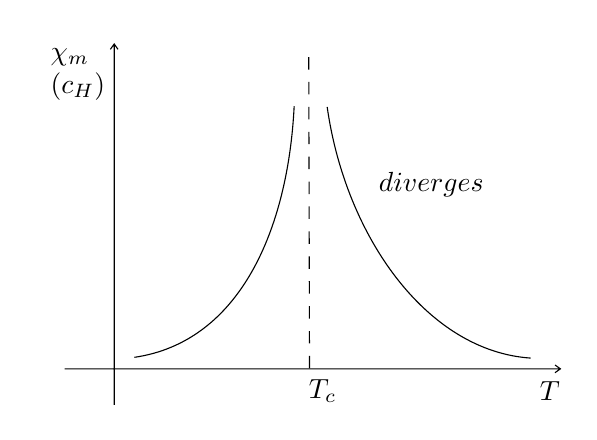
\begin{tikzpicture}[x=0.75pt,y=0.75pt,yscale=-0.37,xscale=0.37]
%uncomment if require: \path (0,476); %set diagram left start at 0, and has height of 476

%Shape: Axis 2D [id:dp5951100625553807]
\draw  (12.61,425) -- (658.18,425)(77.17,2) -- (77.17,472) (651.18,420) -- (658.18,425) -- (651.18,430) (72.17,9) -- (77.17,2) -- (82.17,9)  ;
%Straight Lines [id:da5293875835625754]
\draw  [dash pattern={on 4.5pt off 4.5pt}]  (330.5,19) -- (331.5,425) ;


%Curve Lines [id:da44190238222280653]
\draw    (103.5,410) .. controls (240.5,390) and (303.5,244) .. (311.5,83) ;


%Curve Lines [id:da7750908509461275]
\draw    (619.5,411) .. controls (484.5,402) and (378.5,253) .. (354.5,84) ;



% Text Node
\draw (644.64,453.88) node [scale=1]  {$T$};
% Text Node
\draw (348.49,453.88) node [scale=1]  {$T_{c}$};
% Text Node
\draw (30,36) node [scale=1]  {$ \begin{array}{l}
\chi _{m}\\
( c_{H})
\end{array}$};
\draw (490,185) node [scale=1]  {$diverges$};

\end{tikzpicture}
    \label{fig:} }
\end{minipage}
\begin{minipage}[]{0.5\linewidth}
\centering
\subfloat[][Liquid gas \( k_T = - \frac{1}{V} \pdv{V}{P}  \) ]{
\tikzset{every picture/.style={line width=0.75pt}} %set default line width to 0.75pt

\begin{tikzpicture}[x=0.75pt,y=0.75pt,yscale=-0.37,xscale=0.37]
%uncomment if require: \path (0,476); %set diagram left start at 0, and has height of 476

%Shape: Axis 2D [id:dp5951100625553807]
\draw  (12.61,425) -- (658.18,425)(77.17,2) -- (77.17,472) (651.18,420) -- (658.18,425) -- (651.18,430) (72.17,9) -- (77.17,2) -- (82.17,9)  ;
%Straight Lines [id:da5293875835625754]
\draw  [dash pattern={on 4.5pt off 4.5pt}]  (330.5,19) -- (331.5,425) ;


%Curve Lines [id:da7750908509461275]
\draw    (550.5,348) .. controls (501.5,255) and (456.5,217) .. (395.5,213) .. controls (334.5,209) and (220.5,205) .. (125.5,94) ;


%Shape: Circle [id:dp9976635914729922]
\draw  [fill={rgb, 255:red, 0; green, 0; blue, 0 }  ,fill opacity=1 ] (326,206.5) .. controls (326,204.02) and (328.01,202) .. (330.5,202) .. controls (332.98,202) and (335,204.02) .. (335,206.5) .. controls (335,208.99) and (332.98,211) .. (330.5,211) .. controls (328.01,211) and (326,208.99) .. (326,206.5) -- cycle ;

% Text Node
\draw (644.64,453.88) node [scale=1]  {$T$};
% Text Node
\draw (336.49,449.88) node [scale=1]  {$T_{c}$};
% Text Node
\draw (41,36) node [scale=1]  {$c_{p}$};
% Text Node
\draw (433,163) node   {$flex\ point$};


\end{tikzpicture}
    \label{fig:} }
\end{minipage}
\\
\begin{minipage}[c]{0.5\linewidth}
\centering
\subfloat[][2° order phase transition]{

\tikzset{every picture/.style={line width=0.75pt}} %set default line width to 0.75pt

\begin{tikzpicture}[x=0.75pt,y=0.75pt,yscale=-0.37,xscale=0.37]
%uncomment if require: \path (0,476); %set diagram left start at 0, and has height of 476

%Shape: Axis 2D [id:dp5951100625553807]
\draw  (12.61,425) -- (658.18,425)(77.17,2) -- (77.17,472) (651.18,420) -- (658.18,425) -- (651.18,430) (72.17,9) -- (77.17,2) -- (82.17,9)  ;
%Straight Lines [id:da5293875835625754]
\draw  [dash pattern={on 4.5pt off 4.5pt}]  (330.5,19) -- (331.5,425) ;


%Curve Lines [id:da44190238222280653]
\draw    (103.5,410) .. controls (240.5,390) and (290.5,241) .. (331.5,84) ;


%Curve Lines [id:da7750908509461275]
\draw    (619.5,411) .. controls (484.5,402) and (406.5,367) .. (330.5,213) ;



% Text Node
\draw (644.64,453.88) node [scale=1]  {$T$};
% Text Node
\draw (348.49,453.88) node [scale=1]  {$T_{s}$};
% Text Node
\draw (41,36) node [scale=1]  {$c_{p}$};
% Text Node
\draw (408,185) node   {$jump$};


\end{tikzpicture}
    \label{fig:} }
\end{minipage}
\begin{minipage}[]{0.5\linewidth}
\centering
\subfloat[][Superfluid in \( \lambda\)-transition ]{
\tikzset{every picture/.style={line width=0.75pt}} %set default line width to 0.75pt

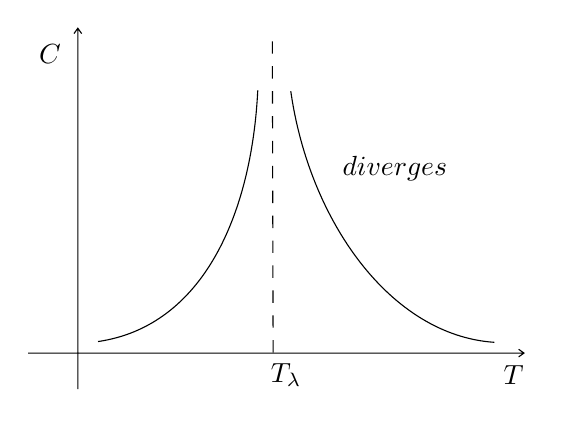
\begin{tikzpicture}[x=0.75pt,y=0.75pt,yscale=-0.37,xscale=0.37]
%uncomment if require: \path (0,476); %set diagram left start at 0, and has height of 476

%Shape: Axis 2D [id:dp5951100625553807]
\draw  (12.61,425) -- (658.18,425)(77.17,2) -- (77.17,472) (651.18,420) -- (658.18,425) -- (651.18,430) (72.17,9) -- (77.17,2) -- (82.17,9)  ;
%Straight Lines [id:da5293875835625754]
\draw  [dash pattern={on 4.5pt off 4.5pt}]  (330.5,19) -- (331.5,425) ;


%Curve Lines [id:da44190238222280653]
\draw    (103.5,410) .. controls (240.5,390) and (303.5,244) .. (311.5,83) ;


%Curve Lines [id:da7750908509461275]
\draw    (619.5,411) .. controls (484.5,402) and (378.5,253) .. (354.5,84) ;



% Text Node
\draw (644.64,453.88) node [scale=1]  {$T$};
% Text Node
\draw (348.49,453.88) node [scale=1]  {$T_{\lambda }$};
% Text Node
\draw (41,36) node [scale=1]  {$C$};
\draw (490,185) node [scale=1]  {$diverges$};

\end{tikzpicture}
    \label{fig:} }
\end{minipage}
\caption{\label{fig:} Description}
\end{figure}
In general, when you are close to \( T_c \), there are singolarities. Now, we can ask, how the curve diverges? What is the behaviour close to the critical point? Power law, so which are the values of these critical exponents?
In order to answer to these questions, let us define:

\begin{bluebox}
\begin{definition}[\textbf{Critical Exponent} (or \emph{Scale Exponent})] \
Define the adimensional parameter \( t \equiv \frac{T-T_c}{T_c} \), the \emph{Critical Exponent} is defined as:
\begin{equation}
  \lambda _{\pm} = \lim_{t \rightarrow 0^{\pm}} \frac{\ln{\abs{F(t)} } }{\ln{\abs{t} } }
  \label{eq:}
\end{equation}
\end{definition}
\end{bluebox}
We note that it behaves like a power low and that
\begin{equation}
  F(t) \overset{t \rightarrow  0^{\pm}}{\sim } \abs{t}^{\lambda _{\pm}}
  \label{eq:}
\end{equation}
Therefore, we can write:
\begin{equation}
  F(t) = A \abs{t}^{\lambda _{\pm}} ( 1 + bt^{\lambda _1}+ \dots) \quad \lambda _1 > 0
  \label{eq:}
\end{equation}
where all other terms are less important.
\begin{bluebox}
\begin{definition}[Exponent]\
\begin{itemize}
\item \textbf{Exponent \( \beta \) }: tells how the order parameter goes to zero.
Consider Figure \ref{fig:3_4_1}, we have \( M \overset{t \rightarrow  0^-}{\sim} (-t)^{\beta }  \). No sense in going from above where it stays 0.

\item \textbf{Exponent \( \gamma _{\pm}  \) }: related to the response function. Consider Figure \ref{fig:3_4_2}, we have \( \chi _T \overset{t \rightarrow 0^{\pm}}{\sim} \abs{t}^{-\gamma _{\pm} }   \). In principle \( \gamma ^+ \neq \gamma ^-  \), but they are the same in reality and we have \( \gamma ^+ = \gamma ^- = \gamma     \).

\item \textbf{Exponent \( \alpha _{\pm} \) }: how specific heat diverges (second order derivative in respect of \emph{T} ). For instance see Figure \ref{fig:3_4_3}, we have \( c_H \sim \abs{t}^{-\alpha _{\pm}}  \).

\item \textbf{Exponent \( \gamma   \)}. In Figure \ref{fig:3_4_4}, \( H \sim \abs{M}^{\delta } \text{sign} (M)  \). Let us ask, how behaves \( \va{M}  \) at the critical point when \( \va{H} \rightarrow 0  \) ?
First of all, we fix \( T=T_c \) and ask what is the value of \( \va{M}(\va{H} ) \). The result is \( M \sim H^{1/\delta } \).
\end{itemize}
\end{definition}
\end{bluebox}



\begin{figure}[h!]
\begin{minipage}[c]{0.5\linewidth}
\centering
\subfloat[][Exponent \( \beta  \) ]{
\tikzset{every picture/.style={line width=0.75pt}} %set default line width to 0.75pt

\begin{tikzpicture}[x=0.75pt,y=0.75pt,yscale=-0.37,xscale=0.37]
%uncomment if require: \path (0,476); %set diagram left start at 0, and has height of 476

%Shape: Axis 2D [id:dp5951100625553807]
\draw  (12.61,425) -- (658.18,425)(77.17,2) -- (77.17,472) (651.18,420) -- (658.18,425) -- (651.18,430) (72.17,9) -- (77.17,2) -- (82.17,9)  ;
%Curve Lines [id:da7750908509461275]
\draw    (470.5,424) .. controls (463.5,331) and (450.5,257) .. (365.5,194) .. controls (280.5,131) and (253.5,117) .. (77.5,92) ;



% Text Node
\draw (644.64,453.88) node [scale=1]  {$T$};
% Text Node
\draw (471.49,448.88) node [scale=1]  {$T_{c}$};
% Text Node
\draw (41,36) node [scale=1]  {$M$};
% Text Node
\draw (306,102) node   {$H=0$};


\end{tikzpicture}
    \label{fig:3_4_1} }
\end{minipage}
\begin{minipage}[]{0.5\linewidth}
\centering
\subfloat[][Exponent \( \gamma_{\pm}  \) ]{
\tikzset{every picture/.style={line width=0.75pt}} %set default line width to 0.75pt

\begin{tikzpicture}[x=0.75pt,y=0.75pt,yscale=-0.37,xscale=0.37]
%uncomment if require: \path (0,476); %set diagram left start at 0, and has height of 476

%Shape: Axis 2D [id:dp5951100625553807]
\draw  (12.61,425) -- (658.18,425)(77.17,2) -- (77.17,472) (651.18,420) -- (658.18,425) -- (651.18,430) (72.17,9) -- (77.17,2) -- (82.17,9)  ;
%Straight Lines [id:da5293875835625754]
\draw  [dash pattern={on 4.5pt off 4.5pt}]  (330.5,19) -- (331.5,425) ;


%Curve Lines [id:da44190238222280653]
\draw    (103.5,410) .. controls (240.5,390) and (303.5,244) .. (311.5,83) ;


%Curve Lines [id:da7750908509461275]
\draw    (619.5,411) .. controls (484.5,402) and (378.5,253) .. (354.5,84) ;



% Text Node
\draw (644.64,453.88) node [scale=1]  {$T$};
% Text Node
\draw (348.49,453.88) node [scale=1]  {$T_{c}$};
% Text Node
\draw (30,36) node [scale=1]  {$\chi$};
\draw (490,185) node [scale=1]  {$H=0$};

\end{tikzpicture}
    \label{fig:3_4_2} }
\end{minipage}
\\
\begin{minipage}[c]{0.5\linewidth}
\centering
\subfloat[][Exponent \( \alpha _{\pm} \) ]{
\tikzset{every picture/.style={line width=0.75pt}} %set default line width to 0.75pt

\begin{tikzpicture}[x=0.75pt,y=0.75pt,yscale=-0.37,xscale=0.37]
%uncomment if require: \path (0,476); %set diagram left start at 0, and has height of 476

%Shape: Axis 2D [id:dp5951100625553807]
\draw  (12.61,425) -- (658.18,425)(77.17,2) -- (77.17,472) (651.18,420) -- (658.18,425) -- (651.18,430) (72.17,9) -- (77.17,2) -- (82.17,9)  ;
%Straight Lines [id:da5293875835625754]
\draw  [dash pattern={on 4.5pt off 4.5pt}]  (330.5,19) -- (331.5,425) ;


%Curve Lines [id:da44190238222280653]
\draw    (103.5,410) .. controls (240.5,390) and (303.5,244) .. (311.5,83) ;


%Curve Lines [id:da7750908509461275]
\draw    (619.5,411) .. controls (484.5,402) and (378.5,253) .. (354.5,84) ;



% Text Node
\draw (644.64,453.88) node [scale=1]  {$T$};
% Text Node
\draw (348.49,453.88) node [scale=1]  {$T_{c}$};
% Text Node
\draw (30,36) node [scale=1]  {$c_{H}$};
\draw (490,185) node [scale=1]  {$H=0$};

\end{tikzpicture}
    \label{fig:3_4_3} }
\end{minipage}
\begin{minipage}[]{0.5\linewidth}
\centering
\subfloat[][Exponent \( \gamma   \) ]{
\tikzset{every picture/.style={line width=0.75pt}} %set default line width to 0.75pt

\begin{tikzpicture}[x=0.75pt,y=0.75pt,yscale=-0.37,xscale=0.37]
%uncomment if require: \path (0,476); %set diagram left start at 0, and has height of 476

%Shape: Axis 2D [id:dp5951100625553807]
\draw  (12.61,242) -- (658.18,242)(329.5,2) -- (329.5,472) (651.18,237) -- (658.18,242) -- (651.18,247) (324.5,9) -- (329.5,2) -- (334.5,9)  ;
%Curve Lines [id:da0018844471566330512]
\draw    (100.5,400) .. controls (207.5,400) and (243.5,430) .. (329.5,242) .. controls (415.5,54) and (537.5,101) .. (571.5,94) ;



% Text Node
\draw (623.64,276.88) node [scale=1]  {$H$};
% Text Node
\draw (497.49,60.88) node [scale=1]  {$T=T_{c}$};
% Text Node
\draw (291,22) node [scale=1]  {$M$};


\end{tikzpicture}
    \label{fig:3_4_4} }
\end{minipage}
\caption{\label{fig:} Description}
\end{figure}




The system displays correlation at very long distance, these goes to the size of the system when \( T \rightarrow T_c \). We are talking about long range correlation. The \emph{correlation function} is \( \xi \sim t^{-\nu } \).
For instance, consider a polymer as in Figure \ref{fig:3_5}.


Consider the \emph{Guggheneim experiment} (see Figure \ref{fig:3_6}), in which we have a liquid-gas. Different sets of data fit the  same function if you rescale \( T/T_c \)
We have
\begin{equation}
  (\rho _l - \rho _c) \sim (-t)^{\beta}
  \label{eq:}
\end{equation}
and \( \beta \sim 1/3 \approx 0.335 \). If you do the same for a string ferromagnetic is 1/3 too. Let us compute:
\begin{equation}
  \begin{cases}
   k_T (c_p-c_v)=T v \alpha ^2 = T v \frac{1}{v^2} \qty(\pdv{v}{T} )^2_P = T \frac{1}{v} \qty(\pdv{v}{T} )^2_P  \\
   \chi _T (c_H-c_M) = T \qty(\pdv{M}{T} )^2
  \end{cases}
\label{eq:}
\end{equation}
with \( c_M \geq 0, \chi _T \geq 0  \) and  \(  c_H \geq \frac{T}{\chi _T} \qty(\pdv{M}{T} )^2 \) because \( c_H = T \). If \( T \rightarrow T_c^-, H=0 \) we have:
\begin{equation}
  \begin{cases}
   c_H \sim (-t)^{-\alpha }\\
   \chi _T \sim (-t)^{-\gamma  }
  \end{cases}
\label{eq:}
\end{equation}
Therefore \( M \sim (-t)^{\beta } \), which implies \( \pdv{M}{T} \sim (-t)^{\beta -1} \). Finally we obtain the \textcolor{blue}{\textbf{RushBrook inequality}}:

\begin{empheq}[box=\myyellowbox]{equation}
\alpha + 2 \beta  + \gamma \geq 2
\end{empheq}










\begin{figure}[h!]
\begin{minipage}[c]{0.5\linewidth}

\subfloat[][Description]{   \centering
\tikzset{every picture/.style={line width=0.75pt}} %set default line width to 0.75pt

\begin{tikzpicture}[x=0.75pt,y=0.75pt,yscale=-0.37,xscale=0.37]
%uncomment if require: \path (0,300); %set diagram left start at 0, and has height of 300

%Curve Lines [id:da3452922115663215]
\draw    (7.5,293) .. controls (206.5,-11) and (350.5,204) .. (645.5,37) ;


%Shape: Circle [id:dp7203554451656493]
\draw  [fill={rgb, 255:red, 0; green, 0; blue, 0 }  ,fill opacity=1 ] (4.86,286.36) .. controls (4.86,282.15) and (8.28,278.73) .. (12.5,278.73) .. controls (16.72,278.73) and (20.14,282.15) .. (20.14,286.36) .. controls (20.14,290.58) and (16.72,294) .. (12.5,294) .. controls (8.28,294) and (4.86,290.58) .. (4.86,286.36) -- cycle ;
%Shape: Circle [id:dp5606402691740692]
\draw  [fill={rgb, 255:red, 0; green, 0; blue, 0 }  ,fill opacity=1 ] (63.86,209.36) .. controls (63.86,205.15) and (67.28,201.73) .. (71.5,201.73) .. controls (75.72,201.73) and (79.14,205.15) .. (79.14,209.36) .. controls (79.14,213.58) and (75.72,217) .. (71.5,217) .. controls (67.28,217) and (63.86,213.58) .. (63.86,209.36) -- cycle ;
%Shape: Circle [id:dp08848917685644386]
\draw  [fill={rgb, 255:red, 0; green, 0; blue, 0 }  ,fill opacity=1 ] (135.86,152.36) .. controls (135.86,148.15) and (139.28,144.73) .. (143.5,144.73) .. controls (147.72,144.73) and (151.14,148.15) .. (151.14,152.36) .. controls (151.14,156.58) and (147.72,160) .. (143.5,160) .. controls (139.28,160) and (135.86,156.58) .. (135.86,152.36) -- cycle ;
%Shape: Circle [id:dp2975813160236622]
\draw  [fill={rgb, 255:red, 0; green, 0; blue, 0 }  ,fill opacity=1 ] (219.86,120.36) .. controls (219.86,116.15) and (223.28,112.73) .. (227.5,112.73) .. controls (231.72,112.73) and (235.14,116.15) .. (235.14,120.36) .. controls (235.14,124.58) and (231.72,128) .. (227.5,128) .. controls (223.28,128) and (219.86,124.58) .. (219.86,120.36) -- cycle ;
%Shape: Circle [id:dp10353996653211406]
\draw  [fill={rgb, 255:red, 0; green, 0; blue, 0 }  ,fill opacity=1 ] (321.86,111.36) .. controls (321.86,107.15) and (325.28,103.73) .. (329.5,103.73) .. controls (333.72,103.73) and (337.14,107.15) .. (337.14,111.36) .. controls (337.14,115.58) and (333.72,119) .. (329.5,119) .. controls (325.28,119) and (321.86,115.58) .. (321.86,111.36) -- cycle ;
%Shape: Circle [id:dp5932331084017816]
\draw  [fill={rgb, 255:red, 0; green, 0; blue, 0 }  ,fill opacity=1 ] (433.86,106.36) .. controls (433.86,102.15) and (437.28,98.73) .. (441.5,98.73) .. controls (445.72,98.73) and (449.14,102.15) .. (449.14,106.36) .. controls (449.14,110.58) and (445.72,114) .. (441.5,114) .. controls (437.28,114) and (433.86,110.58) .. (433.86,106.36) -- cycle ;
%Shape: Circle [id:dp0026977079762487977]
\draw  [fill={rgb, 255:red, 0; green, 0; blue, 0 }  ,fill opacity=1 ] (536.86,82.36) .. controls (536.86,78.15) and (540.28,74.73) .. (544.5,74.73) .. controls (548.72,74.73) and (552.14,78.15) .. (552.14,82.36) .. controls (552.14,86.58) and (548.72,90) .. (544.5,90) .. controls (540.28,90) and (536.86,86.58) .. (536.86,82.36) -- cycle ;
%Shape: Circle [id:dp7071423275830327]
\draw  [fill={rgb, 255:red, 0; green, 0; blue, 0 }  ,fill opacity=1 ] (637.86,37) .. controls (637.86,32.78) and (641.28,29.36) .. (645.5,29.36) .. controls (649.72,29.36) and (653.14,32.78) .. (653.14,37) .. controls (653.14,41.22) and (649.72,44.64) .. (645.5,44.64) .. controls (641.28,44.64) and (637.86,41.22) .. (637.86,37) -- cycle ;

% Text Node
\draw (107,64) node [scale=2.074]  {$N$};


\end{tikzpicture}
    \label{fig:3_5} }
\end{minipage}
\begin{minipage}[]{0.5\linewidth}
\centering
\subfloat[][Description]{   \centering
\tikzset{every picture/.style={line width=0.75pt}} %set default line width to 0.75pt

\begin{tikzpicture}[x=0.75pt,y=0.75pt,yscale=-0.37,xscale=0.37]
%uncomment if require: \path (0,476); %set diagram left start at 0, and has height of 476

%Shape: Axis 2D [id:dp5951100625553807]
\draw  (12.61,425) -- (658.18,425)(77.17,2) -- (77.17,472) (651.18,420) -- (658.18,425) -- (651.18,430) (72.17,9) -- (77.17,2) -- (82.17,9)  ;
%Curve Lines [id:da8602998139648838]
\draw    (540.5,425) .. controls (468.5,-33) and (195.1,-68.97) .. (119.5,424) ;


%Straight Lines [id:da9201699988131803]
\draw  [dash pattern={on 4.5pt off 4.5pt}]  (326.5,67) -- (326.5,425) ;


%Shape: Circle [id:dp2338308227400978]
\draw  [color={rgb, 255:red, 255; green, 0; blue, 0 }  ,draw opacity=1 ][fill={rgb, 255:red, 255; green, 0; blue, 0 }  ,fill opacity=1 ] (124.9,365.08) .. controls (124.9,362.83) and (126.73,361) .. (128.99,361) .. controls (131.24,361) and (133.07,362.83) .. (133.07,365.08) .. controls (133.07,367.34) and (131.24,369.17) .. (128.99,369.17) .. controls (126.73,369.17) and (124.9,367.34) .. (124.9,365.08) -- cycle ;
%Shape: Circle [id:dp8006128175966643]
\draw  [color={rgb, 255:red, 255; green, 0; blue, 0 }  ,draw opacity=1 ][fill={rgb, 255:red, 255; green, 0; blue, 0 }  ,fill opacity=1 ] (146.9,281.08) .. controls (146.9,278.83) and (148.73,277) .. (150.99,277) .. controls (153.24,277) and (155.07,278.83) .. (155.07,281.08) .. controls (155.07,283.34) and (153.24,285.17) .. (150.99,285.17) .. controls (148.73,285.17) and (146.9,283.34) .. (146.9,281.08) -- cycle ;
%Shape: Circle [id:dp23793761340225705]
\draw  [color={rgb, 255:red, 255; green, 0; blue, 0 }  ,draw opacity=1 ][fill={rgb, 255:red, 255; green, 0; blue, 0 }  ,fill opacity=1 ] (170.9,210.08) .. controls (170.9,207.83) and (172.73,206) .. (174.99,206) .. controls (177.24,206) and (179.07,207.83) .. (179.07,210.08) .. controls (179.07,212.34) and (177.24,214.17) .. (174.99,214.17) .. controls (172.73,214.17) and (170.9,212.34) .. (170.9,210.08) -- cycle ;
%Shape: Circle [id:dp6439712554976472]
\draw  [color={rgb, 255:red, 255; green, 0; blue, 0 }  ,draw opacity=1 ][fill={rgb, 255:red, 255; green, 0; blue, 0 }  ,fill opacity=1 ] (205.9,147.08) .. controls (205.9,144.83) and (207.73,143) .. (209.99,143) .. controls (212.24,143) and (214.07,144.83) .. (214.07,147.08) .. controls (214.07,149.34) and (212.24,151.17) .. (209.99,151.17) .. controls (207.73,151.17) and (205.9,149.34) .. (205.9,147.08) -- cycle ;
%Shape: Circle [id:dp09113196346350672]
\draw  [color={rgb, 255:red, 255; green, 0; blue, 0 }  ,draw opacity=1 ][fill={rgb, 255:red, 255; green, 0; blue, 0 }  ,fill opacity=1 ] (264.9,84.08) .. controls (264.9,81.83) and (266.73,80) .. (268.99,80) .. controls (271.24,80) and (273.07,81.83) .. (273.07,84.08) .. controls (273.07,86.34) and (271.24,88.17) .. (268.99,88.17) .. controls (266.73,88.17) and (264.9,86.34) .. (264.9,84.08) -- cycle ;
%Shape: Circle [id:dp9797333610021878]
\draw  [color={rgb, 255:red, 255; green, 0; blue, 0 }  ,draw opacity=1 ][fill={rgb, 255:red, 255; green, 0; blue, 0 }  ,fill opacity=1 ] (322.42,67) .. controls (322.42,64.74) and (324.24,62.92) .. (326.5,62.92) .. controls (328.76,62.92) and (330.58,64.74) .. (330.58,67) .. controls (330.58,69.26) and (328.76,71.08) .. (326.5,71.08) .. controls (324.24,71.08) and (322.42,69.26) .. (322.42,67) -- cycle ;
%Shape: Circle [id:dp6529970568279684]
\draw  [color={rgb, 255:red, 255; green, 0; blue, 0 }  ,draw opacity=1 ][fill={rgb, 255:red, 255; green, 0; blue, 0 }  ,fill opacity=1 ] (407.9,108.08) .. controls (407.9,105.83) and (409.73,104) .. (411.99,104) .. controls (414.24,104) and (416.07,105.83) .. (416.07,108.08) .. controls (416.07,110.34) and (414.24,112.17) .. (411.99,112.17) .. controls (409.73,112.17) and (407.9,110.34) .. (407.9,108.08) -- cycle ;
%Shape: Circle [id:dp9000295114661184]
\draw  [color={rgb, 255:red, 255; green, 0; blue, 0 }  ,draw opacity=1 ][fill={rgb, 255:red, 255; green, 0; blue, 0 }  ,fill opacity=1 ] (452.9,164.08) .. controls (452.9,161.83) and (454.73,160) .. (456.99,160) .. controls (459.24,160) and (461.07,161.83) .. (461.07,164.08) .. controls (461.07,166.34) and (459.24,168.17) .. (456.99,168.17) .. controls (454.73,168.17) and (452.9,166.34) .. (452.9,164.08) -- cycle ;
%Shape: Circle [id:dp9331849007810008]
\draw  [color={rgb, 255:red, 255; green, 0; blue, 0 }  ,draw opacity=1 ][fill={rgb, 255:red, 255; green, 0; blue, 0 }  ,fill opacity=1 ] (485.9,234.08) .. controls (485.9,231.83) and (487.73,230) .. (489.99,230) .. controls (492.24,230) and (494.07,231.83) .. (494.07,234.08) .. controls (494.07,236.34) and (492.24,238.17) .. (489.99,238.17) .. controls (487.73,238.17) and (485.9,236.34) .. (485.9,234.08) -- cycle ;
%Shape: Circle [id:dp5850866249072337]
\draw  [color={rgb, 255:red, 255; green, 0; blue, 0 }  ,draw opacity=1 ][fill={rgb, 255:red, 255; green, 0; blue, 0 }  ,fill opacity=1 ] (514.9,317.08) .. controls (514.9,314.83) and (516.73,313) .. (518.99,313) .. controls (521.24,313) and (523.07,314.83) .. (523.07,317.08) .. controls (523.07,319.34) and (521.24,321.17) .. (518.99,321.17) .. controls (516.73,321.17) and (514.9,319.34) .. (514.9,317.08) -- cycle ;
%Shape: Rectangle [id:dp7713336659871322]
\draw  [color={rgb, 255:red, 47; green, 53; blue, 87 }  ,draw opacity=1 ] (133,323) -- (142.98,323) -- (142.98,332.97) -- (133,332.97) -- cycle ;
%Shape: Rectangle [id:dp5637140961870309]
\draw  [color={rgb, 255:red, 47; green, 53; blue, 87 }  ,draw opacity=1 ] (159,237) -- (168.98,237) -- (168.98,246.97) -- (159,246.97) -- cycle ;
%Shape: Rectangle [id:dp7221266665867194]
\draw  [color={rgb, 255:red, 47; green, 53; blue, 87 }  ,draw opacity=1 ] (190,169) -- (199.98,169) -- (199.98,178.97) -- (190,178.97) -- cycle ;
%Shape: Rectangle [id:dp20263135432878354]
\draw  [color={rgb, 255:red, 47; green, 53; blue, 87 }  ,draw opacity=1 ] (230,109) -- (239.98,109) -- (239.98,118.97) -- (230,118.97) -- cycle ;
%Shape: Rectangle [id:dp7863774801349238]
\draw  [color={rgb, 255:red, 47; green, 53; blue, 87 }  ,draw opacity=1 ] (293,68) -- (302.98,68) -- (302.98,77.97) -- (293,77.97) -- cycle ;
%Shape: Rectangle [id:dp7641507230563557]
\draw  [color={rgb, 255:red, 47; green, 53; blue, 87 }  ,draw opacity=1 ] (370,75) -- (379.98,75) -- (379.98,84.97) -- (370,84.97) -- cycle ;
%Shape: Rectangle [id:dp15909977481521642]
\draw  [color={rgb, 255:red, 47; green, 53; blue, 87 }  ,draw opacity=1 ] (432,132) -- (441.98,132) -- (441.98,141.97) -- (432,141.97) -- cycle ;
%Shape: Rectangle [id:dp5185657164131019]
\draw  [color={rgb, 255:red, 47; green, 53; blue, 87 }  ,draw opacity=1 ] (471,196) -- (480.98,196) -- (480.98,205.97) -- (471,205.97) -- cycle ;
%Shape: Rectangle [id:dp17193812816873077]
\draw  [color={rgb, 255:red, 47; green, 53; blue, 87 }  ,draw opacity=1 ] (502,276) -- (511.98,276) -- (511.98,285.97) -- (502,285.97) -- cycle ;
%Shape: Rectangle [id:dp7377879387307478]
\draw  [color={rgb, 255:red, 47; green, 53; blue, 87 }  ,draw opacity=1 ] (525,361) -- (534.98,361) -- (534.98,370.97) -- (525,370.97) -- cycle ;

% Text Node
\draw (43.5,30.32) node [scale=1]  {$\frac{\rho }{\rho _{c}}$};
% Text Node
\draw (610.64,452.88) node [scale=1]  {$T/T_{c}$};
% Text Node
\draw (355.64,451.88) node [scale=1]  {$1=T_{c} /T_{c}$};

\end{tikzpicture}
    \label{fig:3_6} }
\end{minipage}
\caption{\label{fig:} }
\end{figure}




















\end{document}
